
\section{Signals and properties}

\subsection{Analog and digital signals}

\paragraph{Analog signal} We define a signal is this course as a function of
time or space. For instance $x:\R\rightarrow\dbC$ is a complex 1D signal of time
$t\in\dbR$. $x:\R^2\rightarrow\dbR$ is a 2D image of space $\p\in\dbR^2$.
% \begin{equation}
%     x:\R\rightarrow\dbC= x(t)
%     \label{eq:def_signal}
% \end{equation}

\subsection{Properties of signals}

\paragraph{Causality}\index{Causal signal}
A signal $x(t)$ is causal if 
$$ x(t)=0,\quad \forall x<0 $$

Example: $x(t)= \begin{cases}
0& \text{for } t<0\\
\sin(t)\exp\left(-\frac{t^2}{2}\right) & \text{for } t\geq 0
\end{cases}$

\paragraph{Periodicity}\index{Periodic signal}
A signal $x(t)$ is periodic of period $T_0$ is
$$x(t-kT_0)=x(t),  \forall t\in\mathbb{R}, \forall k\in\mathbb{N}$$      


Example: $x(t)= %\begin{cases}
 % \exp(-\frac{(t-1)^2}{2})&  0<t<T\\
  \exp\left(-\frac{(t-kT_0-1)^2}{2}\right)  \text{ for }kT_0<t<(k+1)T_0,\quad
  \forall k\in\mathbb{N}$
  
\begin{figure}[t]
    \centering
    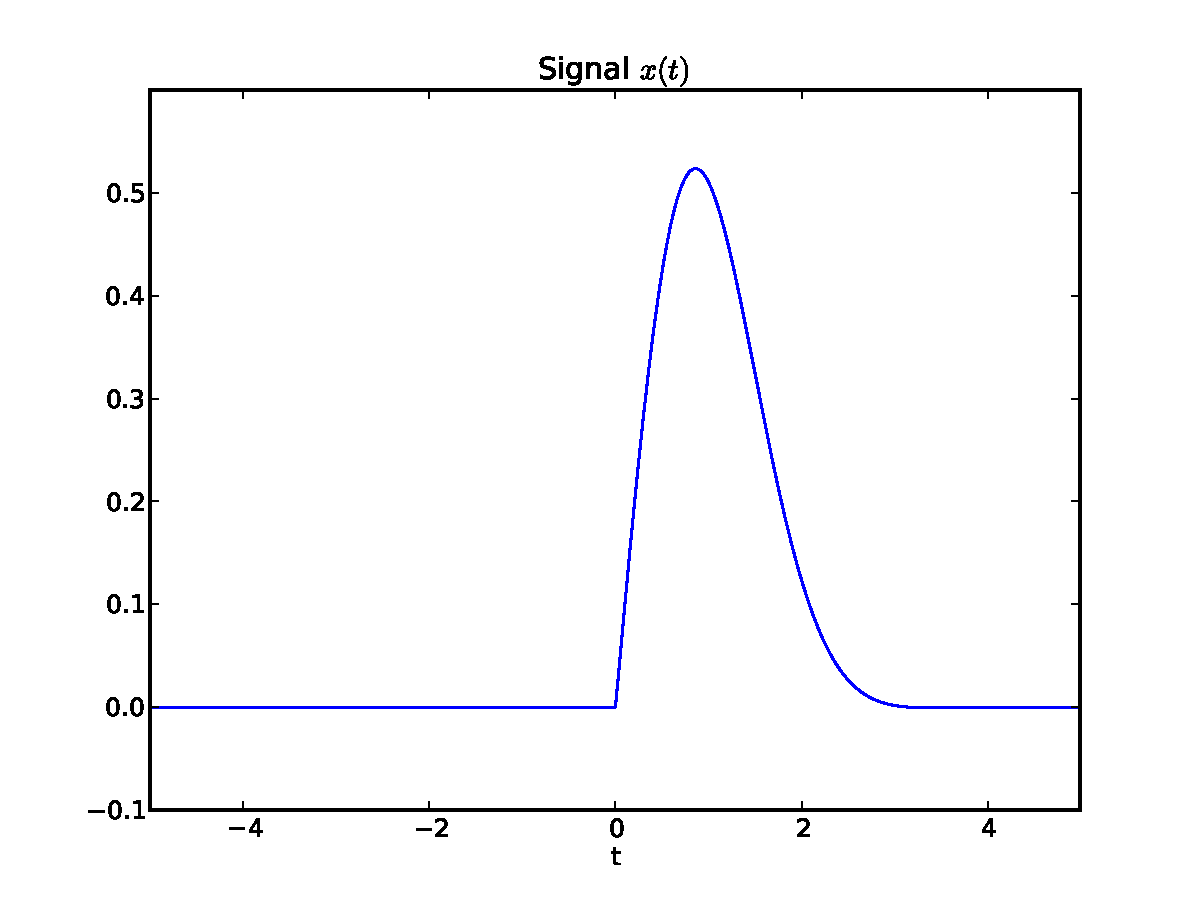
\includegraphics[width=.45\linewidth]{imgs/sig_conv/sig_causal.pdf}
    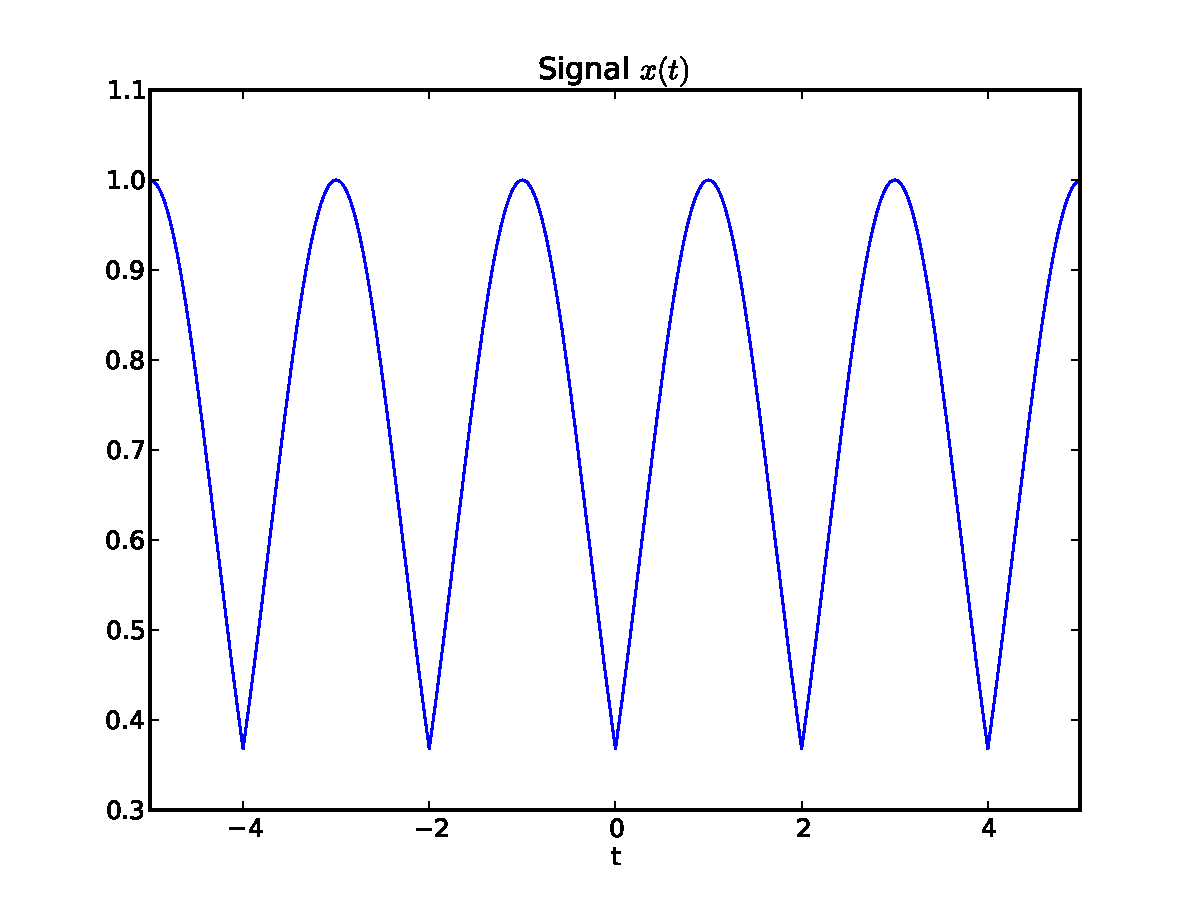
\includegraphics[width=.45\linewidth]{imgs/sig_conv/sig_per.pdf}
    \caption{Examples of Causal signal (left) and periodic signal (right).}
    \label{fig:ex_causal_per}
\end{figure}



\paragraph{Signal in $L_p$ space}\index{$L_p$ space}
$L_p(S)$ is the set of functions whose absolute value to the power of $p$
has a finite integral or equivalently that
\begin{equation}
  \|x\|_p=\int_S |x(t)|^p dt < \infty
  \label{eq:lp_space}
\end{equation}
\begin{itemize}
  \item $L_1(\dbR)$ is the set of absolute integrable functions
  \item $L_2(\dbR)$ is the set of quadratically integrable functions (finite energy)
  \item $L_\infty(\dbR)$ is the set of bounded functions
\end{itemize}

\subsection{Common signals}
\label{sec:common_sig}

\section{Convolution and filtering}
\label{sec:conv_filtering}

\index{Convolution}

\section{Fundamental signal processing problems}
\label{sec:sp_prob}